\documentclass[a4paper, czech]{article}

\title{Úloha č.3: Bipolární tranzistor - V-A charakteristiky}
\author{Karolína Andrea Šebestová}
\date{Datum měření: 14.3.2024}

\usepackage[czech]{babel}
\usepackage{indentfirst}
\usepackage{graphicx}
\usepackage{float}
\usepackage[margin=1.5cm]{geometry}
\usepackage{booktabs}
\usepackage{amsmath}
\usepackage{multirow}
\usepackage{colortbl}

\begin{document}
\maketitle
\section{Teoretický úvod}

Bipolární tranzistor se skládá ze tří různě dotovaných polovodičových oblastí (báze B, emitor E a kolektor C) se dvěma přechody PN v těsném uspořádání. Principiální uspořádání tranzistoru NPN je na Obr. 1.

\begin{figure}[H]
    \centering
    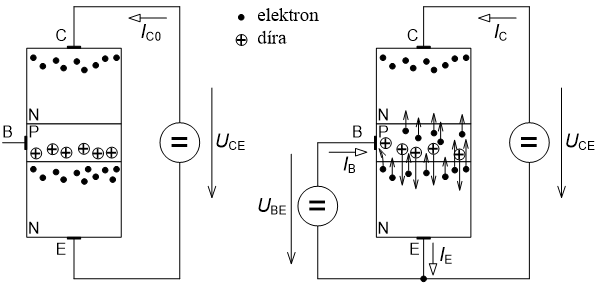
\includegraphics{princip_tranzistoru.png}
    \caption{Princip činnosti tranzistoru}
    \label{obr:1}
\end{figure}

Silně negativně (N) dotovaný emitor emituje elektrony do úzké báze P, kterou většina z elektronů projde a je přitahována kladně polarizovaným kolektorem z polovodiče typu N. Proud elektronů z emitoru do kolektoru lze ovládat velikostí proudu báze. Stejně jako již dříve diskutované prvky i tranzistor je popisován svými AV charakteristikami. K úplnému popisu vlastností tranzistoru (v zapojení SE) slouží čtyři charakteristiky (Obr. 2):

\begin{itemize}
    \item vstupní – závislost vstupního proudu ($I_B$) na vstupním napětí ($U_{BE}$),
    \item výstupní - závislost výstupního proudu ($I_C$) na výstupním napětí ($U_{CE}$),
    \item proudová převodní – závislost výstupního proudu ($I_C$) na proudu vstupním ($I_B$),
    \item zpětná napěťová převodní – závislost vstupního napětí ($U_{BE}$) na napětí výstupním ($U_{CE}$).
\end{itemize}

V praxi jsou nejpoužívanější výstupní charakteristiky.

\begin{figure}[H]
    \centering
    
\includegraphics{soustava_charakteristik.png}
    \caption{Soustava charakteristik bipolárního tranzistoru (NPN) se společným emitorem}
    \label{obr:1}
\end{figure}

\section{Seznam přístrojů}

\begin{enumerate}
    \item Zdroj Agilent E3620A
    \item 2x Multimetr Keysight 34461A
\end{enumerate}

\section{Úkoly měření}

Měření realizujte pomocí zapojení tranzistoru BC546B se společným emitorem na Obr. 3. Vzhledem k tomu, že na pracovišti jsou pouze dva multimetry, které lze využít jako voltmetr či ampérmetr, jsou v jednotlivých úkolech pokyny, kde tyto multimetry zapojit a kde využít např. měření napětí pomocí displeje laboratorního zdroje. Jako zdroje napětí U1 a U2 využijte výstupy V1 a V2 zdroje E3620A.

\begin{figure}[H]
    \centering
    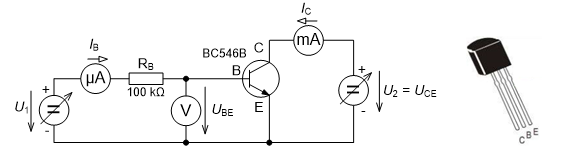
\includegraphics{zapojeni.png}
    \caption{Zapojení pro měření charakteristik bipolárního tranzistoru}
    \label{obr:1}
\end{figure}

\begin{enumerate}
    \item Změřte výstupní charakteristiku tranzistoru, tedy závislost $I_C$ na $U_{CE}$ při $I_B$ = konst. Změřte čtyři křivky pro $I_B = 20; 30; 40; 50 \mu A$. Každou charakteristiku změřte do $U_{CE} = 10 V$, příp. do $I_C = 20 mA$, podle toho, co nastane dříve. Multimetry použijte pro měření proudů $I_B$ a $I_C$. Napětí $U_{CE}$ odečítejte na displeji zdroje E3620A. Voltmetr pro měření $U_{BE}$ zde nebude třeba. Během měření udržujte konstantní proud $I_B$ regulací napětí zdroje $U_1$.
    \item Pro tento úkol ponechte stejné zapojení jako pro předchozí. Změřte proudovou převodní charakteristiku, tedy závislost $I_C$ na $I_B$ při konstantním $U_2 = U_{CE} = 5 V$, které nastavte podle displeje zdroje E3620A. Proud $I_B$ nastavujte od 0 do 70 $\mu A$ s krokem 10 $\mu A$. Proudy $I_B$ a $I_C$ měřte multimetry.
    \item Změřte vstupní charakteristiku, tedy závislost $I_B$ na $U_{BE}$ při konstantním $U_2 = U_{CE} = 5 V$, které nastavte podle displeje zdroje E3620A. Regulací zdroje $U_1$ nastavujte proudy do báze $I_B = 0;1; 2; 5; 10; 20; 30; 50; 70 \mu A$, které měřte multimetrem. Pro tyto proudy měřte druhým multimetrem odpovídající napětí $U_{BE}$. Ampérmetr pro měření $I_C$ zde nebude třeba, nahraďte jej vodičem.
    \item Graficky vykreslete charakteristiky tranzistoru změřené v předchozích bodech. Do grafu se změřenou proudovou převodní charakteristikou dále sestrojte proudovou převodní charakteristiku z hodnot výstupních charakteristik v bodě $U_{CE} = 5 V$ a tyto dvě charakteristiky porovnejte.
\end{enumerate}

\section{Naměřené hodnoty}

V této sekci se nachází tři tabulky.
Vstupní, výstupní a proudové převodní charakteristice náleží po jedné tabulce.
Zpětná napěťová charakteristika měřena nebyla.
V Tabulce 1 je \underline{žlutou} barvou zvýrazněn řádek pro sestrojení druhé proudové převodní charakteristky pro další porovnání. 

Slovní popis symbolů veličin:
$U_{CE}$ - výstupní napětí (kolektor - emitor);
$U_{BE}$ - vstupní napětí (báze - emitor);
$I_B$ - vstupní proud (procházející bází);
$I_C$ - výstupní proud (procházející kolektorem)

\begin{table}[H]
    \centering
    \begin{tabular}{cccccc}
        \toprule
        \multirow{2}{*}{$*$} & \multirow{2}{*}{$U_{CE}\ (V)$} & $I_B = 20 \mu A$ & $I_B = 30 \mu A$ & $I_B = 40 \mu A$ & $I_B = 50 \mu A$ \\
         &  & $I_C\ (mA)$ & $I_C\ (mA)$ & $I_C\ (mA)$ & $I_C\ (mA)$ \\
        \midrule
        1  & 0   & 0     & 0     & 0      & 0      \\
        2  & 0,1 & 0,375 & 0,388 & 0,479  & 0,486  \\
        3  & 0,2 & 0,901 & 2,18  & 2,296  & 1,03   \\
        4  & 0,3 & 3,904 & 3,566 & 3,961  & 4,681  \\
        5  & 0,4 & 4,528 & 4,885 & 5,45   & 6,422  \\
        6  & 0,5 & 5,318 & 6,421 & 6,383  & 7,744  \\
        7  & 0,6 & 5,542 & 7,517 & 6,838  & 9,254  \\
        8  & 0,7 & 5,582 & 7,971 & 9,486  & 10,983 \\
        9  & 0,8 & 5,6   & 8,181 & 10,014 & 11,844 \\
        10 & 0,9 & 5,614 & 8,258 & 10,448 & 12,377 \\
        11 & 1   & 5,622 & 8,292 & 10,821 & 12,877 \\
        12 & 2   & 5,703 & 8,444 & 11,188 & 13,874 \\
        13 & 3   & 5,783 & 8,615 & 11,425 & 14,231 \\
        14 & 4   & 5,848 & 8,748 & 11,688 & 14,557 \\
        \rowcolor{yellow}
        15 & 5   & 5,92  & 8,883 & 11,919 & 14,925 \\
        16 & 6   & 6,045 & 9,028 & 12,122 & 15,272 \\
        17 & 7   & 6,137 & 9,189 & 12,358 & 15,644 \\
        18 & 8   & 6,233 & 9,338 & 12,603 & 16,021 \\
        19 & 9   & 6,312 & 9,514 & 12,834 & 16,396 \\
        20 & 10  & 6,388 & 9,678 & 13,105 & 16,736 \\
        \bottomrule
    \end{tabular}
    \caption{Naměřené hodnoty \underline{výstupní} charakteristiky tranzistoru BC546B (závislost $I_C$ na $U_{CE}$)}
    \label{tab:1}
\end{table}

\begin{table}[H]
    \centering
    \begin{tabular}{cc}
        \toprule
        \multicolumn{2}{c}{$U_2 = U_{CE} = 5V$} \\
        $I_B\ (\mu A)$ & $I_C\ (mA)$ \\
        \midrule
        0  & 0      \\
        10 & 2,97   \\
        20 & 5,949  \\
        30 & 8,951  \\
        40 & 12,106 \\
        50 & 15,186 \\
        60 & 18,337 \\
        70 & 21,525 \\
        \bottomrule
    \end{tabular}
    \caption{Naměřené hodnoty \underline{proudové převodní} charakteristiky tranzistoru BC546B (závislost $I_C$ na $I_B$)}
    \label{tab:1}
\end{table}

\begin{table}[H]
    \centering
    \begin{tabular}{cc}
        \toprule
        \multicolumn{2}{c}{$U_2 = U_{CE} = 5V$} \\
        $I_B\ (\mu A)$ & $U_{BE}\ (V)$ \\
        \midrule
        0  & 0     \\
        1  & 0,573 \\
        2  & 0,603 \\
        5  & 0,636 \\
        10 & 0,661 \\
        20 & 0,687 \\
        30 & 0,701 \\
        50 & 0,726 \\
        70 & 0,753 \\
        \bottomrule
    \end{tabular}
    \caption{Naměřené hodnoty \underline{vstupní} charakteristiky tranzistoru BC546B (závislost $I_B$ na $U_{BE}$)}
    \label{tab:1}
\end{table}

\section{Grafy}

Naměřené hodnoty byly vyneseny do společné soustavy V-A charakteristik, kde jsou křivky jednotlivých charakteristik barevně rozlišeny.
V prvním kvadrantu jsou vyneseny naměřené hodnoty veličin závislosti výstupního proudu $I_C$ na vstupním napětí $U_{CE}$.
Ve druhém kvadrantu jsou vyneseny naměřené hodnoty veličin závislsoti výstupního proudu $I_C$ na vstupním proudu $I_B$.
V třetím kvadrantu jsou vyneseny naměřené hodnoty veličin závislosti vstupního proudu $I_B$ na vstupním napětí $U_{BE}$.

Dále je zde dodatečně vynesena druhá proudová převodní charakteristika z hodnot výstupních charakteristik v bodě $U_{CE} = 5V$, která je v druhém kvadrantu zobrazena \underline{modrou} křivkou.

\begin{figure}[H]
    \centering
    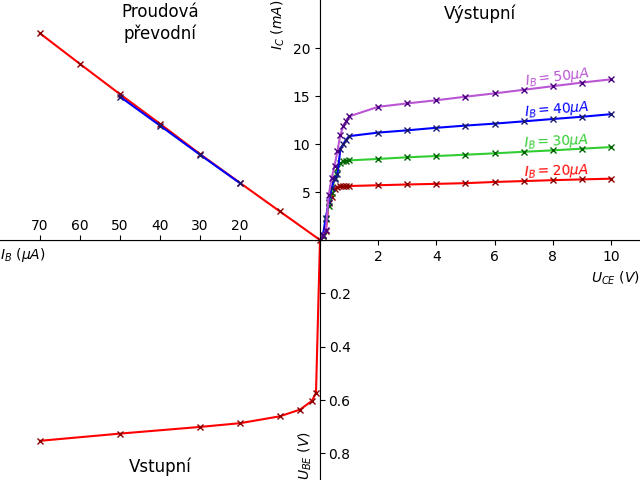
\includegraphics{vach.png}
    \caption{Soustava naméřených charakteristik bipolárního tranzistoru BC546B}
    \label{obr:1}
\end{figure}

\newpage

\section{Závěr}

Jako první jsme měřili výstupní charakteristiku (neboli závislost $I_C$ na $U_{CE}$ při konstantním $I_B$) tranzistoru BC546B.
Výsledné grafické zobrazení charakteristik má tvar připomínající průběh logaritmické funkce.
Měření jsme provedli pro čtyři různé hodnoty vstupního proudu $I_B$.
Na sestrojených charakteristikách pozorujeme, že zvýšením hodnoty $I_B$ se úměrně zvýší i hodnoty výstupního proudu $I_C$ na všech měřených napětích $U_{CE}$.
Za zmínku stojí také, že na jednotlivých výstupních charakteristikách se mírně zvyšovala i jejich strmost.

Dále jsme měřili proudovou převodní charakteristiku tranzistoru, neboli závislost $I_C$ na $I_B$ při konstantním $U_{CE}$.
Měření jsme provedli jen pro několik hodnot $I_B$ a výsledná charakteristika má téměř lineární závislost, což přibližně odpovídá našim očekáváním.

Jako poslední jsme měřili vstupní charakteristiku tranzistoru, tedy závislost $I_B$ na $U_{BE}$ při konstantním $U_{CE}$.
Měření jsme opět provedli jen pro několik hodnot.
Výsledná charakteristika má tvar, který je podobný (avšak inverzní) tvaru naměřených výstupních charakteristik.

Zpětná napěťová převodní charakteristika měřena nebyla.

Dodatečně jsme z hodnot výstupních charakteristik v bodě $U_{CE} = 5V$ sestrojili druhou částečnou proudovou převodní charakteristiku.
Na jejích bodech vynesených do grafu pozorujeme, že se téměř přesně rovná naší primární proudové převodní charakteristice.
Tento jev nás ujišťuje o správnosti měření.
Malá odchylka od primární charakteristiky je nejspíše způsobena drobnými chybami měření.

\end{document}